\documentclass{article}

\usepackage[spanish]{babel}
\usepackage[numbers,sort&compress]{natbib}
\usepackage{graphicx}
\usepackage{url}
\usepackage{amsmath}
\usepackage{hyperref}
\usepackage{listings}
\usepackage[top=30mm, bottom=40mm, left=15mm, right=15mm]{geometry}
\usepackage{color}
\usepackage{subfig}
\usepackage{float}
 
\definecolor{codeblue}{RGB}{0,128,255}
\definecolor{codegray}{rgb}{0.5,0.5,0.5}
\definecolor{codepurple}{rgb}{0.58,0,0.82}
\definecolor{pink}{RGB}{255,26,117}
\definecolor{backcolour}{rgb}{1,1,1}
 
\lstdefinestyle{mystyle}{
    backgroundcolor=\color{backcolour},
    commentstyle=\color{codeblue},
    keywordstyle=\color{pink},
    numberstyle=\tiny\color{codeblue},
    stringstyle=\color{codepurple},
    basicstyle=\footnotesize,
    breakatwhitespace=false,         
    breaklines=true,                 
    captionpos=b,                    
    keepspaces=true,                 
    numbers=left,                    
    numbersep=7pt,                  
    showspaces=false,                
    showstringspaces=false,
    showtabs=false,                  
    tabsize=2
}

\lstset{style=mystyle}

\setlength{\parskip}{2mm}
\setlength{\parindent}{0pt}

\author{Edson Raúl Cepeda Márquez}
\title{Método Monte-Carlo}
\date{\today}

\begin{document}

\maketitle

\section{Objetivo}
El objetivo principal de esta práctica es examinar y analizar los resultados de aplicar el método Monte-Carlo para estimar el resultado de una integral definida.
Se compara los resultados obtenidos con el método Monte-Carlo y Wolfram Alpha con el fin de encontrar el tamaño de muestra  más conveniente para que los resultados sean lo más parecido posible. Esto en medida de cuantos decimales acierta el método. Se gráfica el resultado para así visualizar como afecta el tamaño de la muestra en la cantidad de decimales acertados.

Se hace uso del material de apoyo disponible en la pagina \cite{satu} de la Dra. Elisa Schaeffer, también se hace uso del codigo para el calculo de la integral usando el método Monte-Carlo escrito en el lenguaje de programación R \cite{r}.

\section{Desarrollo}
Se empieza por seleccionar las partes más importantes del código  modificarlas para cumplir el objetivo.
Establecemos un numero de réplicas del experimento y una variación en el tamaño de la muestra que estaremos probando en cada réplica.
\lstinputlisting[language= R, firstline=41, lastline=53]{P5.R}
Dentro de ella se ejecutara la función que calcula la integral.
Los resultados se guardaran en el vector $datos$

Procedemos a establecer el valor esperado para su posterior comparación con los resultados.

\lstinputlisting[language= R, firstline=36, lastline=39]{P5.R}

Se usa la comparación de cadenas de caracteres para comprobar la precisión de las decimales.
Posteriormente se convierten los resultados a cadenas de caracteres para comparar y se guarda en el vector $resultadosstr$.

\lstinputlisting[language= R, firstline=55, lastline=62]{P5.R}

Ahora se calcula la precisión de las decimales.

\lstinputlisting[language= R, firstline=64, lastline=77]{P5.R}.

Se compara los decimales y se incrementa la variable $contador$ en uno cada vez que los resultados aciertan en una decimal.
El ciclo se detiene cuando no acierta pues deja de ser preciso en las siguientes decimales.

\section{Resultados y conclusiones}
Ahora es posible visualizar los resultados.

Antes de dar paso a la conclusión es necesario recalcar que el calculo de la integral en este caso, es solo una aplicación del método Monte-Carlo.

Como podemos observar en la figura \ref{p5} la precisión de los decimales se ve directamente afecta por el tamaño de muestra, es decir, el numero de valores que se generen.
Se alcanza los siete decimales de precisión en las cuatro de las variaciones del tamaño de muestra y tiene una precisión promedio de cinco decimales de exactitud.

Comparando que tan cercanos son los valores obtenidos en el cálculo y con respecto al valor esperado, podemos observar que en promedio los datos se acercaban considerablemente al valor esperado y la menor cantidad de los resultados se alejaban del valor esperado.

Se debe de establecer tamaños de muestra optimo para tener una buena precisión en los cálculos hechos por el método Monte-Carlo.
También es una buena práctica replicar el calculo una cantidad de veces considerable siempre y cuando sé este trabajando con valores aleatorios.



\begin{figure}[H]
\centering
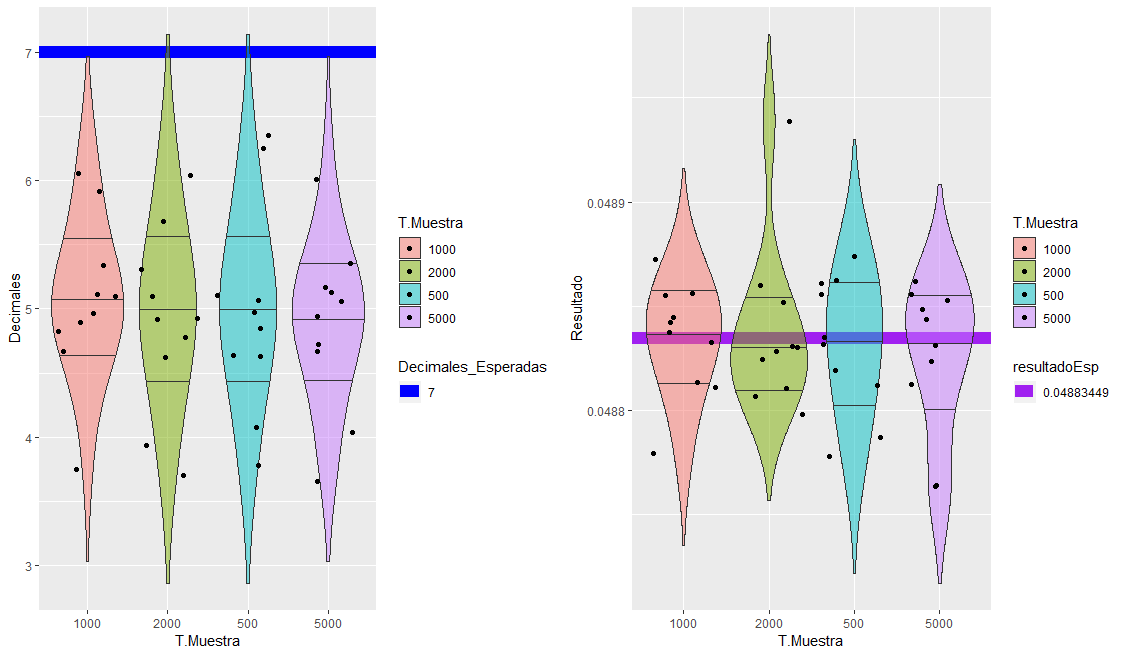
\includegraphics[width=180mm]{P5.png}
\caption{Comparación del tamaño de muestra dependiendo del valor esperado y la cantidad de decimales acertadas en el cálculo de la integral.}
\label{p5}
\end{figure}


\section{Primer reto}
El primer reto consiste en diseñar un experimento para estimar el valor de $\pi$ usando el paralelismo, también se determina la relación matemática entre el número de muestras obtenidas y la precisión de los decimales de los resultados obtenidos.

Se supone un cuadrado el cual contiene un círculo de radio $r$ en su interior.
De esta manera se puede afirmar que el radio del círculo ($r$) sera la mitad de los lados del cuadrado, por lo cual los lados del cuadrado sera dos veces el radio del círculo ($2r$).
Para determinar que área del cuadrado pertenece al círculo se establece la relación en la ecuación \ref{eq1}.

\begin{equation}
\label{eq1}
R = \frac {\pi r^2 } {4 r^2}
\end{equation}

En donde $R$ es la relación del área del cuadrado y el área del círculo y  es el radio , podemos cancelar y despejar $\pi$ para de esta manera obtener la ecuación \ref{eq2} que estaremos utilizando para estimar el valor de $\pi$.

\begin{equation}
\label{eq2}
\pi = {4} * { R}
\end{equation}

Ahora es posible estimar $\pi$ a partir de esta relación.

\lstinputlisting[language= R, firstline=10, lastline=26]{R1P5.R}

Se establece un valor para el radio y se generan números aleatorios entre cero y uno para coordenadas imaginarias de $X$ y $Y$ dentro del cuadrado. Se procede a generar el numero de valores aleatorios especificado en la variable $num$, esto equivale al tamaño de la muestra. Se calcula la distancia pitagórica para así aislar los casos en los que los valores aleatorios estén fuera del área del círculo.
Si un valor coincide dentro del área del círculo entonces la variable $contcirc$ incrementa en uno.

Se calcula $\pi$ con la ecuación \ref{eq1}.
Se toma $R$ como la relación entre el número de veces que los valores aleatorios cayeron dentro del círculo y el total de valores en la muestra.
Se hacen diez réplicas del experimento y se usa una técnica de comparación de cadena de caracteres para encontrar la precisión de decimales de los resultados.

\lstinputlisting[language= R, firstline=27, lastline=60]{R1P5.R}

\begin{figure}[H]
\centering
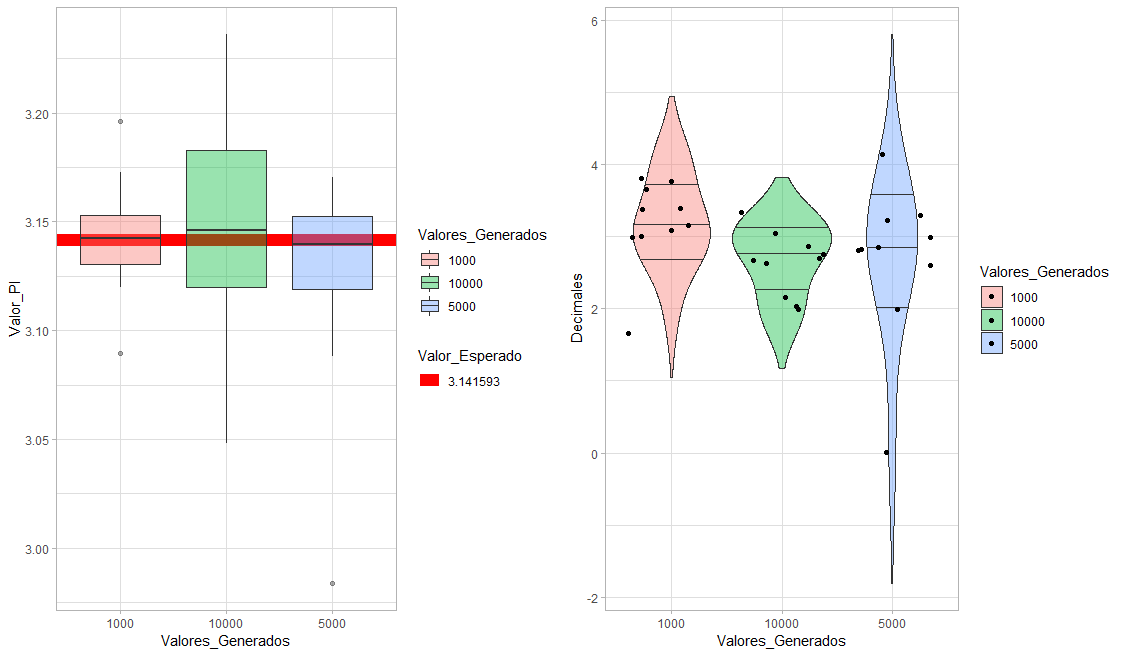
\includegraphics[width=180mm]{Reto1.png}
\caption{Comparación del tamaño de muestra dependiendo del valor esperado y la cantidad de decimales acertadas en la estimación de $\pi$.}
\label{reto}
\end{figure}

Como se puede observar en la figura \ref{reto} los valores seleccionados son adecuados para estimar el valor de $\pi$.
Esto se comprueba viendo que los valores promedio de todas las replicas y el tamaño de muestra, es decir, los valores generados son muy cercanos al valor esperado de $\pi$.Así mismo estos resultados alcanzan hasta 6 decimales de precisión a la hora de estimar el valor de $\pi$.

En la mayoría de los casos usando este método se necesita probar con distintos tamaños de muestra, no siempre usar un tamaño de muestra elevado asegura más precisión en el cálculo.

\begin{thebibliography}{9}

\bibitem{r} 
R:  R Project, 2019
\\\texttt{https://www.r-project.org/}

\bibitem{satu} 
Satu Elisa Schaeffer: Práctica 5: Método Monte-Carlo, 2019
\\\texttt{https://elisa.dyndns-web.com/teaching/comp/par/p5.html}

\bibitem{pi} 
TheCodingTrain: Coding Challenge 95, Approximating the Value of PI, 2018
\\\texttt{https://www.youtube.com/watch?v=5cNnf7e92Ql}

\end{thebibliography}

\end{document}